\documentclass{beamer}
\usetheme{CambridgeUS}
\usepackage{algorithm,algpseudocode}
\usepackage{lmodern, mathtools}
\usepackage{listings}
\usepackage{xcolor}

\definecolor{codegreen}{rgb}{0,0.6,0}
\definecolor{codegray}{rgb}{0.5,0.5,0.5}
\definecolor{codepurple}{rgb}{0.58,0,0.82}
\definecolor{backcolour}{rgb}{0.95,0.95,0.92}

\lstdefinestyle{mystyle}{
    backgroundcolor=\color{backcolour},   
    commentstyle=\color{codegreen},
    keywordstyle=\color{magenta},
    numberstyle=\tiny\color{codegray},
    stringstyle=\color{codepurple},
    basicstyle=\ttfamily\footnotesize,
    breakatwhitespace=false,         
    breaklines=true,                 
    captionpos=b,                    
    keepspaces=true,                 
    numbers=left,                    
    numbersep=5pt,                  
    showspaces=false,                
    showstringspaces=false,
    showtabs=false,                  
    tabsize=2
}

\lstset{style=mystyle}


\title{SC2001 Project 3}
\subtitle{Dynamic Programming}
\author[Hong, Dinh, He]{Hong Jia Yang \and Dinh Pham Minh Anh \and He Qi Xin}
\institute{Team 4}
\date{\today}

\begin{document}

\begin{frame}
	\titlepage
\end{frame}

\begin{frame}
	\frametitle{Outline}
	\tableofcontents
\end{frame}

\section{Environment Specifications}
\begin{frame}
	\frametitle{Environment}
	\begin{itemize}
		\item Software
		\begin{itemize}
			\item C++
			\item MinGW g++ 13.1.0	
			\item Header \texttt{<bits/std++.h>} 
		\end{itemize}
		\item Hardware
		\begin{itemize}
			\item OS: Windows 11 (Home) x86\_64
			\item Processor: Intel(R) Core(TM) i7-10750H (12) @ 2.59 GHz
		\end{itemize}	
	\end{itemize}
	\begin{block}{Note}
		Please refer to \texttt{JamesRobertJohns/team4project3}
	\end{block}
\end{frame}

\section{Recursive Definition}
\subsection{Problem Analysis}
\begin{frame}
	\frametitle{Read the Problem}
	\begin{itemize}
		\item Given a knapsack of capacity of \( C \) weight and \( n \) types of objects, where
	\(
		C, n \in \mathbb{Z}^+
	\)
	\item The \( i^{th} \) object has weight \( w_i \) and profit \( p_i \), where 
		\(
			w_i, p_i \in \mathbb{Z}^+
		\)
		\begin{itemize}
			\item This makes the problem simpler 
			\item If values can be negative, we can displace the terms by \( - min(\{w_i\}) \) and \( - min(\{p_i\}) \) correspondingly such that they become \emph{non-negative} 
			\item The optimal filling will be the same, but optimal value will be adjusted accordingly
		\end{itemize}	
	\item There are \emph{unlimited} supplies of each type of objects
		\begin{itemize}
			\item \textbf{Unbounded} - We can use the object more than once
			\item Similar concept in Coin Change II 
		\end{itemize}	
	\item Find the \emph{largest} total profit of any set of the object that fits in the knapsack
		\begin{itemize}
			\item Greedy doesn't work - consider any counter example
		\end{itemize}
	\end{itemize}
\end{frame}

\subsection{Intuition}
\begin{frame}
\frametitle{Intuition}
	\begin{itemize}
		\item There are only two choices
		\item Either we \textbf{take} the \( i^{th} \)  item 
			\begin{itemize}
				\item We gain \( p_i \)
				\item Capacity is \(C := C - w_i \)  
				\item We can continue this process for the \( i^{th} \) item
				\item This can continue so long as the capacity is sufficient 
			\end{itemize}
		\item Or we \textbf{don't take} the \( i^{th} \)  item
			\begin{itemize}
				\item Our profit stays the same
				\item Capacity stays the same 
				\item We move on to the \( i+1^{th} \) item
			\end{itemize}
		\item We want to find the \textbf{maximum} of the choices 
	\end{itemize}	
\end{frame}

\subsection{Formal Definition}
\begin{frame}
	\frametitle{Formalise the Problem}
	We want to find 
	\[
		max\left( \sum_{ i = 0 }^{ n - 1 }{ p_ix_i }  \right) 
	\]
	Given the \textbf{constraint}  
	\[
		\sum_{ i = 0 }^{ n -1 }{ w_ix_i } \leq C 
	\]
	Where
	\[
		x_i \geq 0, x_i \in \mathbb{Z}^+
	\]
\end{frame}

\begin{frame}
	\frametitle{Formalise the Problem}
	Let \( dp(n, C) \) denote the function describing this relationship
	\begin{itemize}
		\item Base case 
			\begin{align*}	
				dp(n, 0) &= 0\\
				dp(0, C) &= 0 
			\end{align*}	
		\item Taking the \( i^{th} \) item, the state transition to
			\[
				dp(i, C-w_i) + p_i
			\]
		\item Not taking the \( i^{th} \) item, the state transition to
			\[
				dp(i+1, C)
			\]
		\item We want to find the maximum value, given by
			\[
				max(dp(i+1, C), dp(i, C-w_i) + p_i)
			\]
	\end{itemize}
\end{frame}

\begin{frame}
	\frametitle{Recursive Definition}
	\[
		dp(n, C) = \begin{cases}
					0 & \text{if } n = 0 \text{ or } C = 0 \\
					max(dp(i+1, C), dp(i, C-w_i)) & \text{otherwise} 
				\end{cases}
	\]
\end{frame}

\section{Sub-problem Graph}
\begin{frame}
	\frametitle{2 parameters}
	\begin{figure}
		\centering
		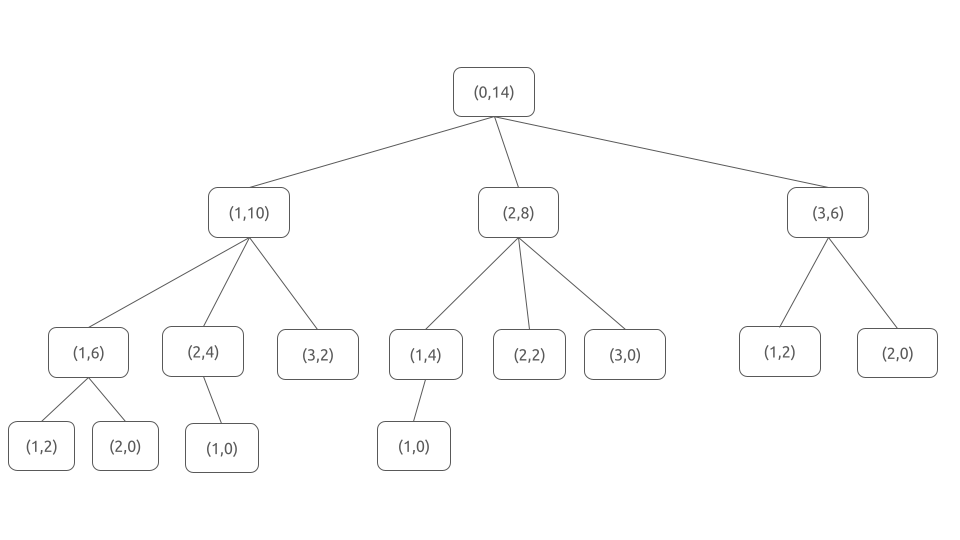
\includegraphics[width=0.95\textwidth]{asset/1.png}
		\caption{sub-problem graph for 2 parameters, current item and current capacity}
	\end{figure}	
\end{frame}

\begin{frame}
	\frametitle{2 parameters}
	\begin{figure}
		\centering
		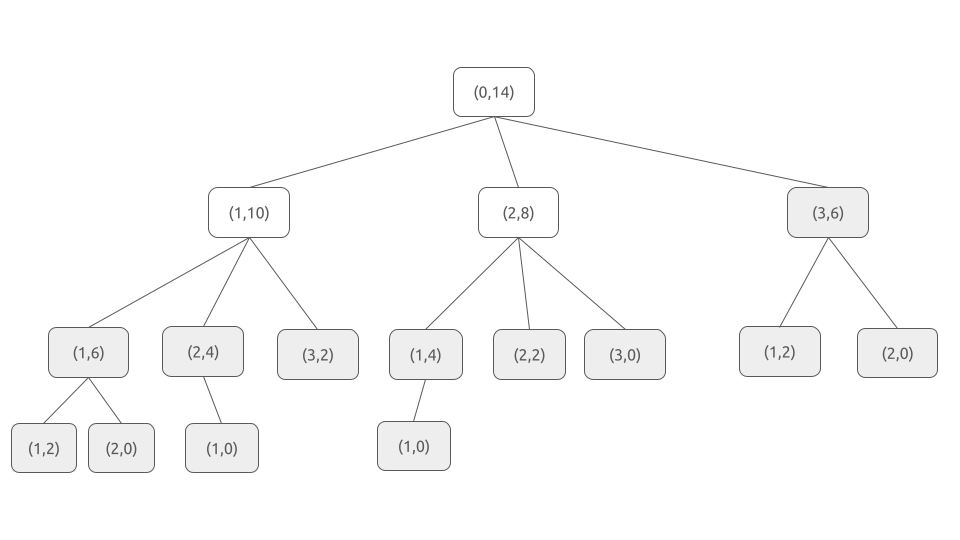
\includegraphics[width=0.95\textwidth]{asset/2.png}
		\caption{repeated sub problems - optimal solution for \( C \) comes from weight \( C-1 \) }
	\end{figure}	
\end{frame}

\begin{frame}
	\frametitle{1 parameter}
	\begin{figure}
		\centering
		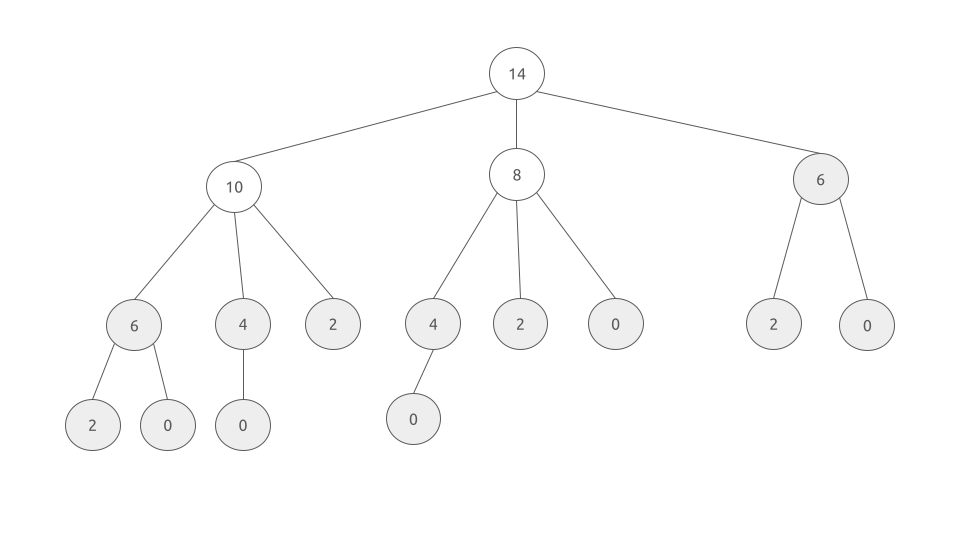
\includegraphics[width=0.95\textwidth]{asset/3.png}
		\caption{Since infinite supplies, tracking item is irrelevant, one parameter suffice}
	\end{figure}	
\end{frame}

\begin{frame}
	\frametitle{Condensed Graph}
	\begin{figure}
		\centering
		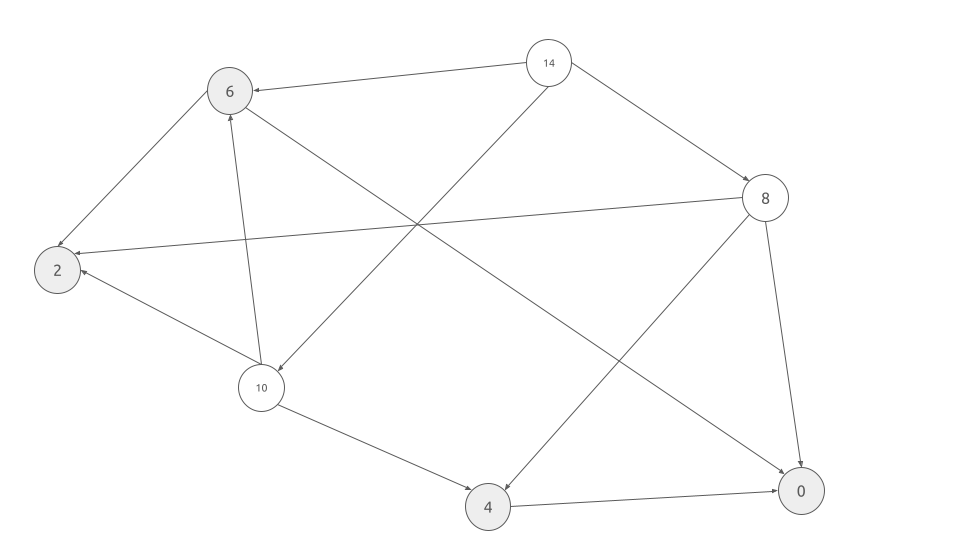
\includegraphics[width=0.95\textwidth]{asset/4.png}
		\caption{Overlapping sub-problems which fulfil the optimal substructure property}
	\end{figure}
\end{frame}


\section{Algorithm}
\begin{frame}
	\frametitle{Complexity Analysis}
	\begin{itemize}
		\item The time complexity will be \( O(nC) \) 		
			\begin{itemize}
				\item The outer loop executes \( n \) times in worst case (rows)
				\item The inner loop executes \( C \) times in worst case (columns)
				\item Bottom up indexing will take constant time 
			\end{itemize}
		\item Using 2D array, the space complexity will be
			\[
				O((n+1)(C+1)) = O(nC)
			\]
		\item Using 1D array, the space complexity will be
			\[
				O(C+1) = O(C)
			\]
	\end{itemize}
\end{frame}

\subsection{Pseudo code}
\begin{frame}
		\begin{algorithm}[H]
		\caption{bottom up dp}
		\begin{algorithmic}[1]
			\Function{dp}{$i, C$}
			\State initialise \( A \) with \( n+1 \) rows and \( C+1 \) columns
			\State \( A \gets \{0\} \) 
			\For{ \( i \gets 1 \) to \( n \) }				
			\For{ \( j \gets 1 \) to \( C \) }
			\If{ $w[i-1] > j$ }
			\State $A[i][j] \gets A[i-1][j]$ 
			\Else
			\State \( A[i][j] \gets max(A[i-1][j], A[i][j-w[i]]+p[i-1]) \) 
			\EndIf
			\EndFor
			\EndFor
			\EndFunction
		\end{algorithmic}
	\end{algorithm}	
\end{frame}

\subsection{Implementation}
\begin{frame}
	\frametitle{2D Array}
  \lstinputlisting[language=C++]{asset/dp.cpp}
\end{frame}

\begin{frame}
	\frametitle{1D Array (Space Optimised)}
  \lstinputlisting[language=C++]{asset/dpp.cpp}
\end{frame}

\begin{frame}
  \frametitle{IO specification}
  Let the input be \texttt{.text} files, such that the first line is capacity $C$, and second line is number of objects $n$. The third and fourth lines are the respective values of $w_i$ and $p_i$  for the $i^{th}$ object, space delimited
  \begin{itemize}
    \item Test case 1 can be represented as \newline
        14\newline
        3\newline
        4 6 8\newline
        7 6 9\newline
    \item Test case 2 can be represented as \newline
        14\newline
        3\newline
        5 6 8\newline
        7 6 9\newline
  \end{itemize}
\end{frame}

\begin{frame}
	\frametitle{main}
  \lstinputlisting[language=C++]{asset/main.cpp}
\end{frame}

\begin{frame}
  \frametitle{output}
  \begin{itemize}
    \item Output of \texttt{./a < ../data/input1.txt}
      \begin{itemize}
        \item 21
      \end{itemize}
    \item Output of \texttt{./a < ../data/input2.txt}
      \begin{itemize}
        \item 16 
      \end{itemize}
	 \item You can specify your own input files
  \end{itemize}
\end{frame}

\end{document}
